\textcolor{blue}{\textit{Pierre JACQUOT}}

In order to get the GPS coordinates of each robots we decided to use the \textit{GPRMC} sentence send by the GPS's emitter. The exemple below show the structure of a \textit{GPRMC} sentence : \
\begin{center}
\begin{tabular}{|m{0.05\linewidth}|m{0.06\linewidth}|m{0.07\linewidth}|m{0.07\linewidth}|m{0.08\linewidth}|m{0.07\linewidth}|m{0.07\linewidth}|m{0.04\linewidth}|m{0.08\linewidth}|m{0.1\linewidth}|m{0.07\linewidth}|}
\hline
    081836 & A & 3751.65 & S & 14507.36 & E & 000.0 & 360.0 & 130998,01 & 011.3 & E*62  \\ \hline
     UTC & Data status & Latitude & N or S & Longitude & E or W & Speed (knots) & Track made good &  UT Date & Magnetic Variation & E or W and Checksum \\ \hline

\end{tabular}
\end{center}
The most valuable data are the latitude, the longitude, the speed over ground (in knots) ant the time stamp. In order to get those different data, we used the python package pynmea, which allows to easily get and parse a GPS sentence. \\
However, the longitude and latitude obtained using this specific sentence have a particular structure that we had to changed to make them easier to manipulate and compute in our algorithm. The example below show how the longitude and latitude are originally formatted :
\
\begin{itemize}
  \item Longitude  : \textit{12311.12,W} which means Longitude 123 degree. 11.12 min West
  \item Latitude : \textit{4916.45,N} which means Latitude 49 degree 16.45 min North
\end{itemize}

In order to ease the computation, our program automatically convert the longitude and latitude in degrees, take into account the cardinal direction associated with each coordinates.
These cardinal directions North and South for the latitude and East and West for the longitude, let us know respectively on which side of the Greenwich (or prime) meridian we are located and on which side of the equator we are located. As a matter of fact, we will have in Brest a "negative" latitude and a positive longitude, due to our positioning regarding the equator and Greenwich meridian.\\

Our program not only give the coordinates in degrees but also convert them into UTM (Universal Transverse Mercator) coordinates. This new set of coordinates allow a localisation of the robot in a flat local coordinates system and maybe more easy to use as they are just decimal numbers. The UTM system itself, consist in a subdivision of the world in different sectors which can be consider as flat, and with a specific system of coordinates.
The figure below show the subdivision of France: \

\begin{center}
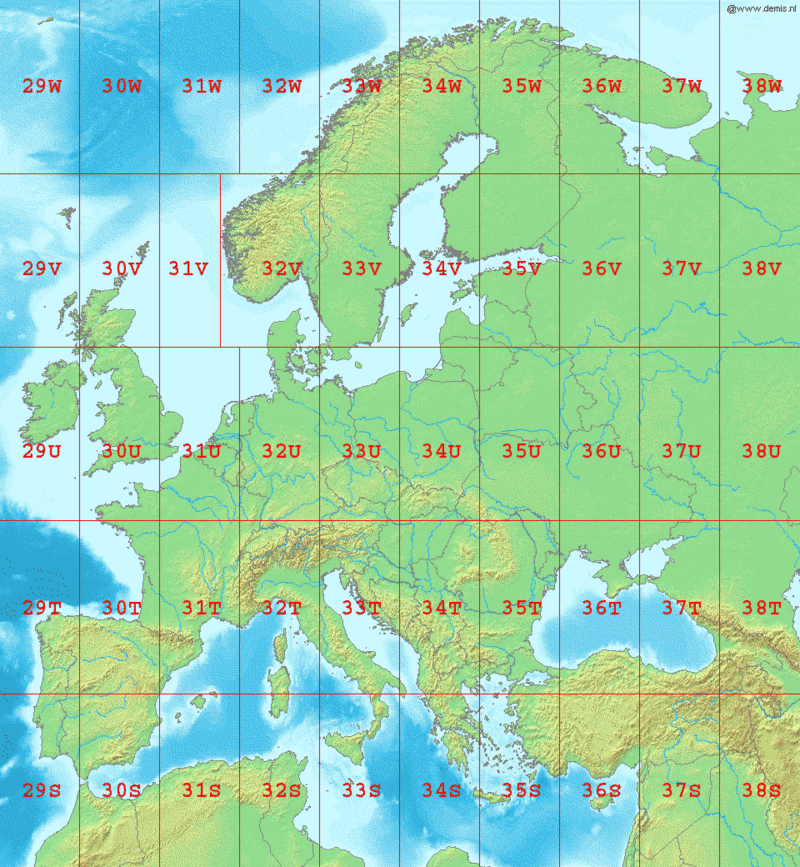
\includegraphics[scale=0.2]{secteurUTM.png} 
\captionof{figure}{Secteur UTM}
\label{fig1}
\end{center}

This figure show that we are currently in the sector 30. Whereas,in order to compute UTM coordinates, we need first to choose a geodesic system representing the Earth. For this project we chose the WGS-84 system which is most commonly used.



